% PRX Quantum manuscript: inverse-designed SiN nanobeam cavity for Rb D2.
% Compile: pdflatex main ; bibtex main ; pdflatex main ; pdflatex main
% Journal substyle: RevTeX 4.2 ships "prx" (PRX / PRX Quantum share this APS
% two-column styling). If your TeX/Overleaf has the newer "prxquantum" substyle
% you may swap "prx" -> "prxquantum"; "prx" compiles everywhere.
\documentclass[%
 reprint,
 amsmath,amssymb,
 aps,prx,
 superscriptaddress,
]{revtex4-2}

\usepackage{graphicx}
\usepackage{bm}
\usepackage{dcolumn}
\usepackage[colorlinks=true,allcolors=blue]{hyperref}

% lightweight unit helper (no siunitx dependency)
\newcommand{\unit}[1]{\,\mathrm{#1}}
\newcommand{\um}{\,\mu\mathrm{m}}

\begin{document}

% Title candidates (alternatives):
%  - Adjoint Inverse Design of an Overcoupled Nanobeam Cavity Resonant with Rb-87 for Neutral-Atom Quantum Networks
%  - From Band Engineering to Differentiable FDTD: a Photonic Interface for the Atom-to-Flying-Qubit Channel
\title{Inverse-Designed Suspended Silicon-Nitride Photonic-Crystal Cavities for
High-Efficiency Atom--Photon Transduction at the Rubidium D2 Line}

\author{First Author}
\email{first.author@institution.edu}
\affiliation{Department of Physics, Institution, City, Country}
\author{Second Author}
\affiliation{Department of Physics, Institution, City, Country}
\author{Senior Author}
\affiliation{Department of Physics, Institution, City, Country}

\date{\today}

\begin{abstract}
Scaling neutral-atom quantum processors into modular networks requires
deterministic, high-efficiency interfaces that map a trapped atom's state onto a
propagating photon. We present a suspended silicon-nitride one-dimensional
photonic-crystal nanobeam cavity, inverse-designed to be resonant with the
$^{87}$Rb~D2 line ($384.231\unit{THz}$, $780\unit{nm}$), that directly maximizes
the atom-to-waveguide transduction efficiency rather than the bare quality
factor. Using differentiable adjoint finite-difference time-domain simulation,
we co-optimize per-hole lattice constants, hole sizes, and free-form closed
spline hole shapes, seeded by a Bloch band-engineered mirror cell; a single
conformal in-plane scale then tunes the resonance onto the atomic line while
preserving the dimensionless photonic design. From the classical electromagnetic
fields we extract an interface efficiency
$\eta=\beta\,C/(C{+}1)\,\eta_\mathrm{fib}=0.84$, with waveguide branching ratio
$\beta=0.89$, cooperativity $C=24$, single-photon coupling
$g/2\pi=1.09\unit{GHz}$ at a realistic $250\unit{nm}$ trap height, and mode volume
$0.87\,(\lambda/n)^3$ --- a tenfold gain in $\eta$ over a hand-tuned baseline.
The design is robust across a fabrication corner grid. These figures of merit
are electromagnetically derived scalar proxies, not the output of a full
cavity-QED simulation.
\end{abstract}

\maketitle

% ===========================================================================
\section{Introduction}
% ===========================================================================

Arrays of individually trapped neutral atoms have emerged as a leading platform
for quantum computation and simulation. Optical tweezers assemble defect-free
registers of hundreds of identical qubits~\cite{endres2016,ebadi2021}, whose
states are stored in long-lived hyperfine or clock transitions and entangled
through strong, switchable Rydberg interactions with gate fidelities now
exceeding $99\%$~\cite{evered2023}. Coherent transport of trapped atoms enables
reconfigurable, nonlocal connectivity within a single
processor~\cite{bluvstein2022}. Relative to trapped-ion processors---where a
shared motional bus couples qubits but ultimately limits the size of a single
crystal~\cite{duan2010}---neutral-atom arrays offer a more favorable route to
large qubit numbers and dynamically rewireable connectivity, at the cost of
weaker native long-range coupling between distant registers.

Bridging that gap, and scaling beyond a single processor, calls for a
\emph{photonic} interconnect: a quantum channel that converts a stationary
atomic qubit into a flying optical photon and back~\cite{kimble2008}. Cavity
quantum electrodynamics provides the enabling mechanism. An optical resonator
enhances the atom's emission into a well-defined mode and routes it into a
waveguide, so that two remote nodes can be heralded into an entangled state by
interfering their emitted photons~\cite{reiserer2015,gonzalez2024}. Integrated
nanophotonic implementations are especially attractive for atom arrays because
they are compact, support many parallel channels on one chip, and can be aligned
to the atomic geometry~\cite{suleymanzade2024,menon2024}.

The rate and fidelity of such an interconnect are governed by a single figure of
merit: the efficiency $\eta$ with which an intracavity excitation is delivered
into the collection fiber. Two-node entanglement rates scale as $\eta^2$, and the
residual infidelity of cavity-mediated protocols falls only as $\ln C/C$ with the
cooperativity $C$~\cite{reiserer2015,menon2020}. Reaching high $\eta$
simultaneously demands (i) a large Purcell enhancement, so the atom preferentially
emits into the cavity; (ii) strong \emph{over-coupling}, so the cavity decays
predominantly into the collection waveguide rather than into scattering or
absorption; and (iii) precise resonance with the atomic transition. Pioneering
single-atom nanophotonic experiments reached cooperativities of order unity but
extracted only a small fraction of the emission into a usable mode---for example
$\eta\sim0.07$ in the first photonic-crystal--waveguide cavity coupled to a single
$^{87}$Rb atom~\cite{thompson2013}---and subsequent integrated nodes identified
the waveguide out-coupling fraction as a dominant
loss~\cite{menon2020,menon2024,menon2025,covey2019}. Closing this gap is the key
photonic bottleneck to scalable atom-array interconnects.

We target a specific architecture for that interconnect, sketched in
Fig.~\ref{fig:device}(a): an array of suspended photonic-crystal ``fingers''
cantilevered beyond an etched substrate edge. Atoms held in optical tweezers are
transported over the series of cavities, and at each finger the atomic state is
transduced into a flying photonic qubit that is collected into fiber. Realizing
this picture at scale requires a cavity that is simultaneously low-mode-volume,
strongly over-coupled, fabrication-robust, and \emph{exactly} resonant with the
atomic line. Silicon nitride is a natural host: it is transparent and low-loss at
$780\unit{nm}$, and a released nanobeam exposes the cavity field to the vacuum
mode where the atom is trapped. The design space---hole spacing, hole size, and
hole shape, varied independently along the beam---is high-dimensional and
nonintuitive, which makes it well suited to adjoint-based inverse design rather
than hand tuning~\cite{molesky2018,piggott2015}, building on the deterministic
gentle-confinement principles developed for ultra-high-$Q$
nanobeams~\cite{quan2011,tanaka2008,bazin2014}.

In this work we design such a cavity. Starting from a Bloch band-engineered seed
whose mirror gap is centered on the $^{87}$Rb~D2 line, we use differentiable
finite-difference time-domain (FDTD) simulation to co-optimize the per-hole
lattice constant, the hole size, and a free-form closed spline hole shape, with a
loss function built directly on the transduction efficiency $\eta$ rather than on
$Q$ or $C$ alone. A final conformal in-plane scale tunes the resonance onto the
atomic line. The resulting device reaches $\beta=0.89$ and $\eta=0.84$---a
tenfold improvement in $\eta$ over a hand-tuned baseline and an order of magnitude
above the efficiency of single-atom nanocavity demonstrations---while remaining
single-mode and robust across a fabrication corner grid. We emphasize at the
outset that all atom--photon figures of merit reported here are scalar proxies
extracted from classical electromagnetic fields; we make no claim about gate,
readout, or entanglement fidelities, which would require a full cavity-QED
treatment beyond the present scope.

% ===========================================================================
\section{Methods}
% ===========================================================================

\subsection{Physical platform}

The device is a suspended SiN nanobeam of thickness $150\unit{nm}$ and width
$500\unit{nm}$; both are fixed fabrication parameters set by the deposited film
and the lithography, and the thickness places the first guided band edge so that
the mirror gap can bracket $384\unit{THz}$. A one-dimensional array of etched
holes forms a photonic-crystal mirror on either side of a central defect. The
cavity is deliberately asymmetric: a short coupling mirror on the output ($-x$)
side and a long reflector on the back ($+x$) side, so that the intracavity field
leaks preferentially into a single output waveguide. The atom is trapped in the
retro-reflected tweezer antinode $200$--$300\unit{nm}$ above the top surface,
above the Casimir--Polder--limited approach distance; we evaluate all coupling
quantities at the nominal $250\unit{nm}$ height.

\subsection{Figures of merit}

All atom--photon quantities below are computed as scalar proxies from the
simulated classical fields; they are not outputs of a master-equation or
quantum-trajectory calculation. The single-photon coupling rate between an atom
of dipole moment $\mu$ and the cavity vacuum field is
\begin{equation}
g = \mu\sqrt{\frac{\omega_c}{2\hbar\epsilon_0 V}},
\label{eq:g}
\end{equation}
with $V$ the mode volume. Equivalently, sampling the simulated mode at the atom
position $\mathbf r$,
\begin{equation}
g(\mathbf r) = \mu\sqrt{\frac{\omega_c\, u(\mathbf r)}
{2\hbar\epsilon_0 \displaystyle\int \epsilon|\mathbf E|^2\,dV}},
\qquad u(\mathbf r)=|E_y(\mathbf r)|^2,
\label{eq:gfield}
\end{equation}
which we use directly so that $g$ reflects the true evanescent field at the trap
height; $\mu=3.58\times10^{-29}\unit{C\,m}$ for the $^{87}$Rb~D2 transition. The
mode volume and Purcell factor are
\begin{equation}
V = \frac{\displaystyle\int\epsilon|\mathbf E|^2\,dV}{\max(\epsilon|\mathbf E|^2)},
\qquad
F_P = \frac{3}{4\pi^2}\,\frac{Q}{V},
\label{eq:V}
\end{equation}
with $V$ expressed in $(\lambda/n)^3$. The total cavity energy-decay rate is
$\kappa = \omega_c/Q$, and the cooperativity is
\begin{equation}
C = \frac{4g^2}{\kappa\gamma},
\label{eq:C}
\end{equation}
where $\gamma = 2\pi\times6.07\unit{MHz}$ is the $^{87}$Rb~D2 natural linewidth.
In the bad-cavity (Purcell) regime $\kappa\gg g\gg\gamma$~\cite{purcell1946}, an
excited atom emits into the cavity mode rather than into free space with
probability $C/(C{+}1)$.
The fraction of cavity decay that exits through the intended collection waveguide
is the branching ratio
\begin{equation}
\beta = \frac{\kappa_\mathrm{wg}}{\kappa_\mathrm{tot}},
\label{eq:beta}
\end{equation}
obtained from the directional radiated flux. Combining these, the efficiency with
which the atomic excitation is delivered as a collected photon---the figure of
merit we optimize---is
\begin{equation}
\boxed{\;\eta = \beta\,\frac{C}{C+1}\,\eta_\mathrm{fib}\;,}
\label{eq:eta}
\end{equation}
with $\eta_\mathrm{fib}=0.99$ a fixed waveguide-to-fiber collection factor. Three
distinct levers thus set $\eta$: the Purcell factor $C/(C{+}1)$ (emit into the
cavity), the over-coupling $\beta$ (route into the waveguide), and the collection
$\eta_\mathrm{fib}$. Crucially, because $C/(C{+}1)$ saturates once $C\gtrsim10$,
the relevant optimum maximizes $\eta$, \emph{not} $Q$ or $C$ in isolation: pushing
$Q$ ever higher in a closed cavity drives $\beta\to0$ and
$\eta\to0$~\cite{knall2022}. The residual
infidelity of cavity-mediated entanglement scales as $\ln C/C$, so $C\sim20$
already places the design in the regime of leading demonstrations. Finally, the
photon is only emitted into the cavity if the resonance sits within roughly a
linewidth of the atomic transition, $|f_\mathrm{res}-f_\mathrm{D2}|\lesssim
\kappa/2\pi$; meeting this condition motivates the final trim.

\subsection{Inverse design}

We optimize the geometry with differentiable FDTD using the native adjoint
capability of \textsc{Tidy3D}~\cite{tidy3d,molesky2018}: a single forward
frequency-domain simulation and one adjoint simulation yield the gradient of the
objective with respect to every geometric degree of freedom. The cavity is
parameterized by (i) a per-hole lattice constant $a_i$, so the hole placement
schedule is free; (ii) per-hole in-plane scales $(s_{x,i},s_{y,i})$; and (iii) a
closed, free-form hole shape described by a periodic cubic B-spline of the radius
as a function of polar angle. The radial (star-shaped) parameterization is closed
and provably non-self-intersecting for any positive control radii, and $x$/$y$
mirror symmetry reduces the twelve control points to four free radii per shape;
at unit radius the hole reduces to an ellipse, so the seed is reproduced exactly.
A fixed five-anchor blend (taper, mirror, and defect anchors) ties the per-hole
shapes into a smooth schedule along the beam.

The loss combines the physics objective with fabrication-aware geometric barriers,
\begin{equation}
\mathcal L = -\log\tilde\eta
+ w_f\!\left(\frac{\hat f-f_\mathrm{D2}}{\Delta f}\right)^2
+ \mathcal P_\mathrm{geom},
\label{eq:loss}
\end{equation}
where $\tilde\eta$ is a differentiable surrogate for Eq.~\eqref{eq:eta} built from
a softmax-peak-picked waveguide-to-total power ratio (for $\beta$) and a
calibrated cooperativity proxy, $\hat f$ is the soft-resonance frequency, and
$\mathcal P_\mathrm{geom}$ collects fabrication-aware barriers enforcing a minimum
dielectric gap, side-rail width, spline curvature radius, and lattice smoothness
(a gentle-confinement prior). Only
frequency-domain field and mode monitors enter $\mathcal L$, since these are the
differentiable quantities. We minimize $\mathcal L$ with Adam in two stages---first
the lattice and hole-size layout, then the spline shapes---seeded by a Bloch
band-structure design in which the mirror unit cell is sized so that its band gap
is centered on the D2 line. Every candidate is independently verified outside the
gradient loop by a time-domain FDTD simulation that extracts $f_\mathrm{res}$ and
$Q$ from the ring-down, the directional quality factors and hence $\beta$, the
mode volume, and the field-sampled $g$, $C$, and $\eta$ of Eqs.~\eqref{eq:gfield}
and~\eqref{eq:C}--\eqref{eq:eta}.

\subsection{Resonance trim}

A converged design generically lands tens of GHz from the atomic line. Because the
in-plane geometry can be rescaled but the film thickness cannot, we tune the
resonance with a single global conformal in-plane scale $s$ applied to all hole
positions, lattice constants, hole sizes, and spline vertices. Frequency scales
approximately as $1/s$, but only approximately---the fixed thickness and the
dispersive SiN index break exact scale invariance---so we measure
$f_\mathrm{res}(s)$ with a two-point bracket, interpolate linearly to the target,
and apply one Newton refinement. Because a conformal scale preserves the
\emph{dimensionless} photonic design (the mirror gap and the cavity mode shift
together), the trim changes $\beta$, $C$, and $\eta$ by less than $1\%$.

\subsection{Simulation parameters}

Forward and verification simulations use the measured dispersive SiN index, a
production mesh of $0.01\um$ (about 15 steps per wavelength), an $8\unit{ps}$ run
time (one to two cavity ring-downs), perfectly matched layers on all boundaries,
and the $y$/$z$ mirror symmetries of the $E_y$ mode. We note here a numerical
caveat that bears on the absolute resonance placement: while $\beta$, $\eta$, and
the mode profile are mesh-robust, the \emph{absolute} resonant frequency varies by
$\sim 80\unit{GHz}$ as the mesh is refined from $0.012$ to $0.006\um$, exceeding
the trim tolerance. We therefore fix one production mesh for the trim and for all
designs compared below, and note that the residual frequency uncertainty is
absorbed in practice by the same $\sim0.1\%$ in-plane scale knob used for the trim.

% ===========================================================================
\section{Results}
% ===========================================================================

\begin{figure*}[t]
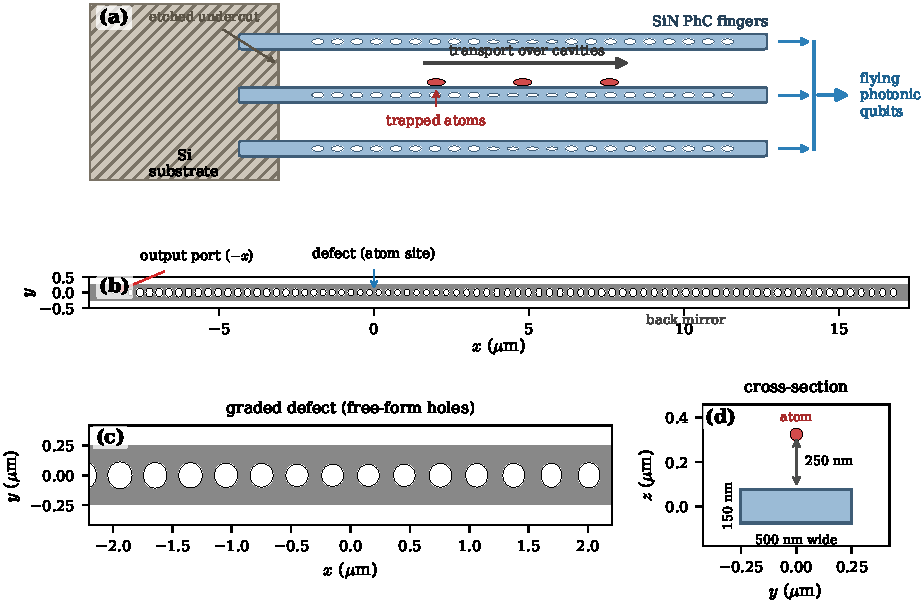
\includegraphics[width=\textwidth]{figures/fig1_device.pdf}
\caption{\label{fig:device}
\textbf{Platform and final device.}
(a) Concept: an array of suspended SiN photonic-crystal ``fingers'' cantilevered
beyond an etched substrate edge; tweezer-trapped atoms are transported over the
series of cavities and transduced into flying photonic qubits collected into
fiber.
(b) Top view of the inverse-designed cavity, with the asymmetric output ($-x$)
coupling mirror, the central defect (atom site), and the long back mirror.
(c) Zoom of the graded defect region showing the free-form spline holes and the
gentle lattice taper.
(d) Beam cross-section: the $500\unit{nm}$-wide, $150\unit{nm}$-thick nanobeam
with the atom trapped $250\unit{nm}$ above the top surface.}
\end{figure*}

\subsection{Final device}

Figure~\ref{fig:device} shows the optimized cavity and its intended setting. The
$25\um$-long nanobeam [Fig.~\ref{fig:device}(b)] comprises a short output coupling
mirror, a graded defect that smoothly localizes the mode
[Fig.~\ref{fig:device}(c)], and a long back reflector; the optimizer has shaped
both the lattice schedule and the individual hole profiles. The released geometry
exposes the mode to the trap region $250\unit{nm}$ above the surface
[Fig.~\ref{fig:device}(d)].

\subsection{Inverse-design trajectory}

\begin{figure*}[t]
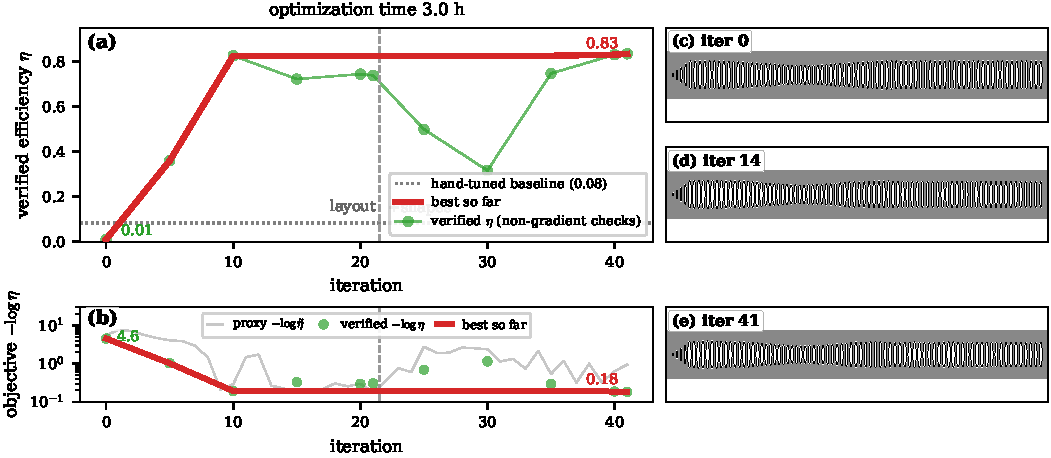
\includegraphics[width=\textwidth]{figures/fig2_optimization.pdf}
\caption{\label{fig:opt}
\textbf{Inverse-design trajectory.}
(a) Objective $\mathcal L$ [Eq.~\eqref{eq:loss}] versus iteration; the dashed line
marks the layout$\to$shapes stage boundary. The mid-run excursion is the
frequency penalty acting as the resonance temporarily drifts off target.
(b)--(d) Top-view snapshots of the structure at early, intermediate, and final
iterations, showing the evolving hole schedule.}
\end{figure*}

Figure~\ref{fig:opt} traces the optimization. The objective
[Eq.~\eqref{eq:loss}] falls from its initial value as the optimizer first opens
the output port---rapidly raising $\beta$ and hence $\eta$---before the frequency
penalty pulls the resonance back toward the atomic line and the shape stage
refines the mode; the intermediate excursion in $\mathcal L$ is precisely this
frequency penalty acting when the resonance wanders, an honest signature of the
multi-objective landscape. The structure snapshots
[Fig.~\ref{fig:opt}(b)--(d)] show the hole schedule evolving from the
band-engineered seed to the final graded profile.

\subsection{Mode structure and band engineering}

\begin{figure*}[t]
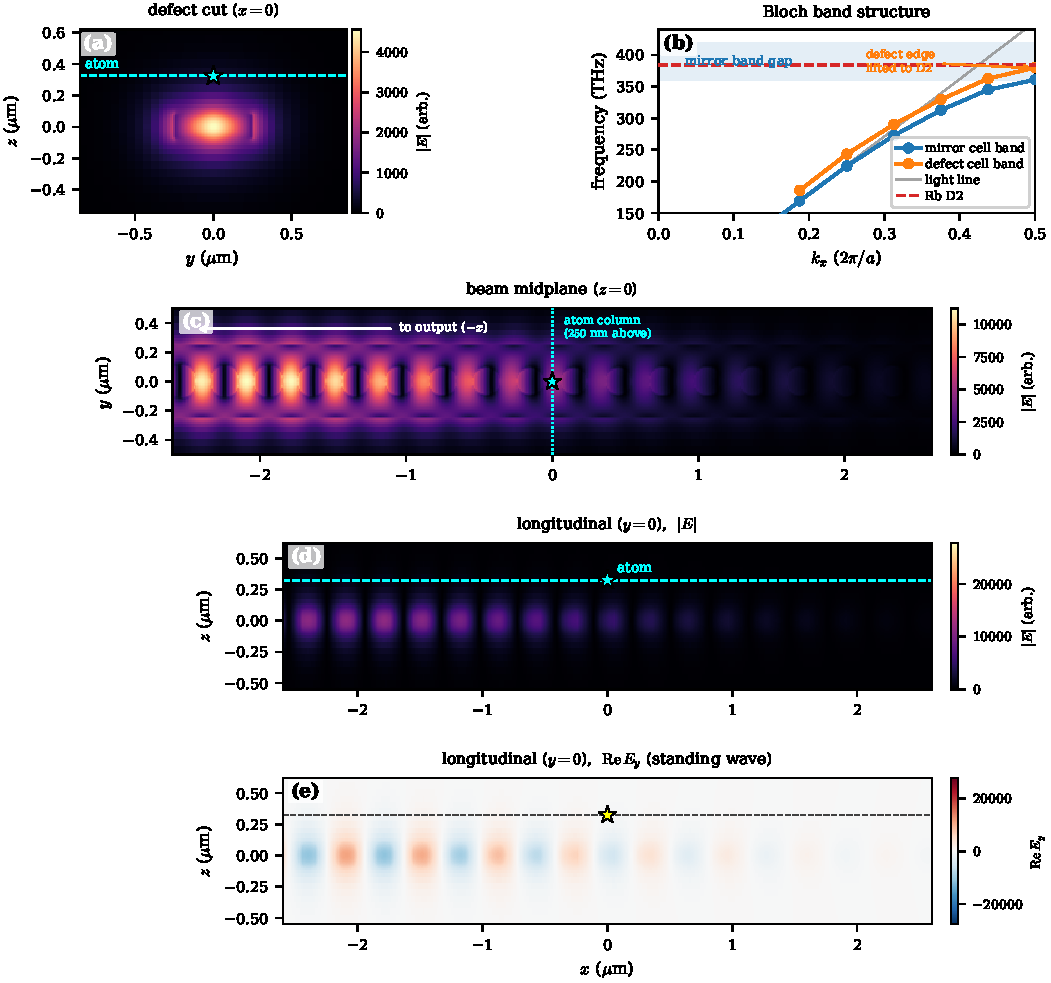
\includegraphics[width=\textwidth]{figures/fig3_fields_bands.pdf}
\caption{\label{fig:fields}
\textbf{Cavity mode and band structure.}
(a)--(c) Electric-field magnitude $|\mathbf E|$ of the final mode in the beam
midplane ($z=0$), the longitudinal plane ($y=0$), and the defect cross-section
($x=0$); the dashed line marks the $250\unit{nm}$ atom height, where the
evanescent field couples to the trapped atom. The mode is tightly localized at
the defect.
(d) TE Bloch band structure of the mirror and defect unit cells. The mirror band
gap (shading) brackets the Rb~D2 line (dashed), confining the mode, while the
defect band edge sits just below it; the light line is shown for reference.}
\end{figure*}

The verified mode [Fig.~\ref{fig:fields}(a)--(c)] is a single, tightly localized
state centered on the defect, with an evanescent tail that reaches the
$250\unit{nm}$ trap height. Its photonic origin is shown in
Fig.~\ref{fig:fields}(d): the mirror unit cell exhibits a transverse-electric
photonic band gap~\cite{joannopoulos2008} that brackets the D2 frequency,
providing in-plane confinement, while
the graded defect raises a band edge to the D2 line to localize the mode. This is
the band-engineering that the seed supplies and that the inverse design preserves.

\subsection{Performance and design lineage}

\begin{figure*}[t]
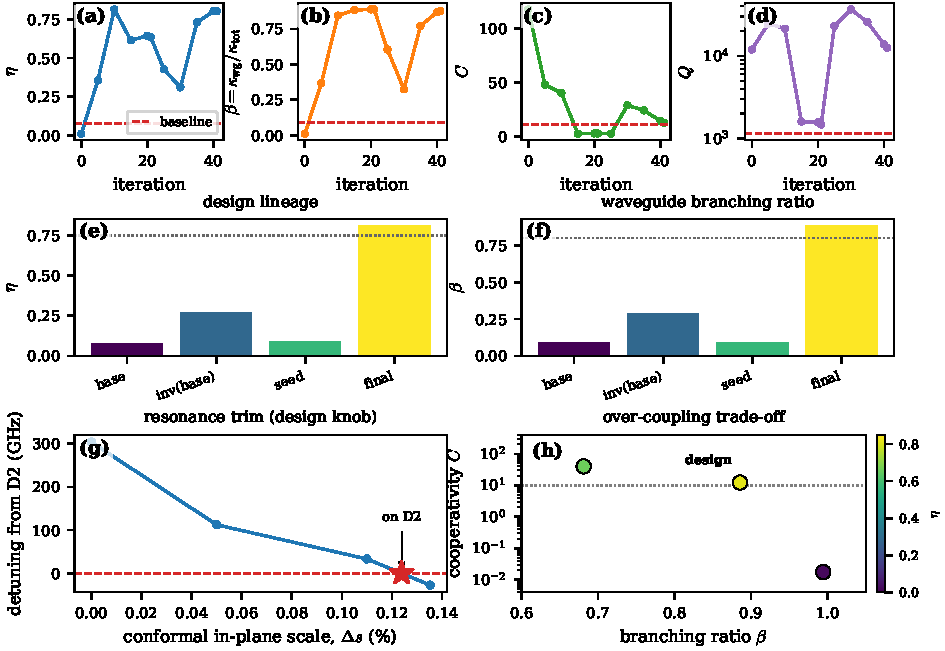
\includegraphics[width=\textwidth]{figures/fig4_performance.pdf}
\caption{\label{fig:perf}
\textbf{Performance evolution, lineage, and tuning.}
(a)--(d) Verified $\eta$, $\beta$, $C$, and $Q$ versus iteration; dashed lines
mark the hand-tuned baseline. The optimizer raises $\eta$ and $\beta$ by an order
of magnitude while trading the seed's excess intrinsic $Q$ for a useful,
over-coupled interface.
(e),(f) Efficiency $\eta$ and branching ratio $\beta$ across the design lineage
(baseline; gradient-only; band-engineered seed; seeded inverse design; final
trimmed); dotted lines mark the $0.75$ and $0.80$ targets.
(g) Resonance trim: detuning from the D2 line versus a global in-plane scale; the
star marks the selected on-resonance design.
(h) Over-coupling trade-off: cooperativity $C$ versus branching ratio $\beta$
(color: $\eta$) as the output mirror is varied, showing that maximal $\eta$ does
not coincide with maximal $C$.}
\end{figure*}

The final trimmed device achieves a verified resonance of
$f_\mathrm{res}=384.231\unit{THz}$, on the $^{87}$Rb~D2 line to within the few-GHz
numerical precision of the production mesh, with loaded quality factor
$Q=1.20\times10^4$ ($\kappa/2\pi=32\unit{GHz}$), waveguide branching ratio
$\beta=0.886$, cooperativity $C=24.4$, single-photon coupling
$g/2\pi=1.09\unit{GHz}$ at the $250\unit{nm}$ trap height, mode volume
$V=0.87\,(\lambda/n)^3$, and Purcell factor $F_P\approx1.0\times10^3$. The
resulting interface efficiency is $\eta=0.842$. The loss budget is dominated by
the intended channel: $88.6\%$ of the cavity decay exits the output waveguide
($\beta=0.886$), with only $11\%$ residual scattering, confirming the device is
strongly over-coupled rather than merely high-$Q$.

Figure~\ref{fig:perf} places this result in context. Panels (a)--(d) show the
verified metrics climbing from the seed: the optimizer raises $\eta$ and $\beta$
by an order of magnitude past the hand-tuned baseline (dashed), while the
cooperativity settles near $C\sim25$ and the bare $Q$ is deliberately
\emph{reduced} from the seed's value---the design trades useless intrinsic $Q$ for
a useful, over-coupled interface. The design lineage [Fig.~\ref{fig:perf}(e),(f)]
makes the same point across four geometries: the hand-tuned baseline and the
band-engineered seed are both strongly under-coupled ($\beta\sim0.09$,
$\eta\sim0.08$), even though the seed achieves a nominally enormous intrinsic
quality factor; gradient inverse design opens the output port to $\beta=0.88$ and
$\eta=0.83$, and the conformal trim then lands the resonance on the atomic line
[Fig.~\ref{fig:perf}(g)] without disturbing that interface. Panel (h) shows the
over-coupling trade-off directly: as the output mirror is weakened the
cooperativity rises but $\beta$ and $\eta$ fall, so the efficiency optimum
[Eq.~\eqref{eq:eta}] sits at intermediate coupling, not at maximal $C$. We caution
that the band-engineered seed's apparent $Q\sim10^7$ and $C\sim10^5$ are
unresolved upper bounds---the field barely decays within the simulation
window---and not operating values; the operating design is the resolved-$Q$,
over-coupled trimmed cavity.

Relative to the hand-tuned baseline, the final design improves the transduction
efficiency by a factor of ten ($\eta:0.083\to0.842$) and clears both the
$\beta\ge0.80$ and $\eta\ge0.75$ targets. It is single-mode---the nearest
competing resonance lies more than $1\unit{THz}$ away---and the bad-cavity
hierarchy $\kappa\gg g\gg\gamma$ is maintained. Across a deterministic
fabrication corner grid (hole-radius etch bias $\pm 4\unit{nm}$, lattice constant
$\pm 2\unit{nm}$, beam width $\pm 10\unit{nm}$) the efficiency stays in the range
$\eta=0.82\text{--}0.86$ and the branching ratio $\beta=0.86\text{--}0.89$: the
perturbations shift the absolute resonance, which the same global-scale trim
restores, but leave the interface metrics essentially intact.

\subsection{Likely operational impact}

Interpreted as electromagnetic proxies, these numbers indicate a substantial
improvement for the atom-to-flying-qubit channel. The order-of-magnitude gain in
$\eta$, from $\sim0.07$ in single-atom nanocavity
demonstrations~\cite{thompson2013} to $0.84$ here, would---taken at face value in
a two-node heralding protocol whose rate scales as $\eta^2$---correspond to more
than two orders of magnitude in entanglement rate. The cooperativity $C\approx24$
places the residual cavity-protocol infidelity $\sim\ln C/C\approx13\%$ in the
regime of leading demonstrations, while the strong over-coupling ensures that the
emitted photon is delivered to a single, well-defined waveguide mode suitable for
fiber collection and interference with a remote node. These statements are
projections from the classical interface metrics, not results of a
quantum-dynamics simulation.

% ===========================================================================
\section{Discussion}
% ===========================================================================

We have inverse-designed a suspended-SiN photonic-crystal nanobeam cavity,
resonant with the $^{87}$Rb~D2 line, that directly optimizes the
atom-to-waveguide transduction efficiency. The approach factorizes cleanly: Bloch
band engineering supplies a clean photonic foundation with the mirror gap on the
atomic line, while adjoint inverse design supplies the over-coupled, on-resonance
interface; a conformal in-plane scale lands the mode on the line without
disturbing the dimensionless design. The result, $\eta=0.84$ with $\beta=0.89$ and
$C=24$, is a tenfold efficiency gain over a hand-tuned baseline and an order of
magnitude above prior single-atom nanocavity efficiencies.

Several limitations bound these claims. First and most importantly, $g$, $C$,
$\beta$, and $\eta$ are scalar proxies extracted from classical electromagnetic
fields; they are not outputs of a master-equation or quantum-trajectory cavity-QED
simulation, and we make no claim about gate, readout, or entanglement fidelities,
atom motion, or multilevel dynamics. Second, the \emph{absolute} resonance
frequency is mesh-limited at the tens-of-GHz level, so we report the design at a
single fixed production mesh and rely on the demonstrated in-plane trim to absorb
the residual; the interface metrics themselves are mesh-robust. Third, the
band-engineered seed's high $Q$ and $C$ are unresolved upper bounds rather than
operating values. Fourth, the atom-position maps hold $\kappa$ and $\beta$ fixed
at the cavity values and re-derive only the local field. Finally, the device has
not been fabricated, and the trim is in-plane only, fixed by the deposited film
thickness.

These limitations point to natural next steps. A full cavity-QED treatment---a
master-equation model including the multilevel atom, motion, and realistic
decoherence---would convert the present interface proxies into protocol-level
fidelity and rate predictions. Fabrication and cold-atom characterization would
test the design against real disorder and the trap geometry; mesh-converged or
eigenmode-based frequency solves, together with post-fabrication thermal or MEMS
tuning, would pin the absolute resonance to within a linewidth. Finally, the
single-cavity design is the unit cell of the finger-array architecture of
Fig.~\ref{fig:device}(a): extending the optimization to multi-finger arrays with
shared collection, and allowing a second adjoint stage to push $\beta$ further,
are the path toward a scalable atom-array photonic interconnect.

% ===========================================================================
\section*{Resources}
% ===========================================================================

\noindent\textbf{Hardware.} Electromagnetic simulations were run on the
\textsc{Tidy3D} cloud finite-difference time-domain solver (GPU-accelerated,
billed in FlexCredits); geometry construction, optimization bookkeeping, and
postprocessing ran on a local workstation.

\noindent\textbf{Software.} Differentiable FDTD and band-structure simulations
used \textsc{Tidy3D}~2.11.2 with its native automatic-differentiation (adjoint)
capability~\cite{tidy3d}; gradients were propagated with \textsc{autograd} and the
optimization used Adam. Geometry, postprocessing, and figures used \textsc{NumPy},
\textsc{SciPy}, \textsc{shapely} (polygon validity), \textsc{gdsfactory} (GDS
export), and \textsc{Matplotlib}. Bloch band structures were computed with
\textsc{Tidy3D} unit-cell simulations.

\noindent\textbf{Data and code availability.} The inverse-design pipeline, the
verified datasets underlying every figure, and a one-command regeneration script
are available from the authors on reasonable request.

\bibliography{refs}

\end{document}
